\chapter{Person Detection, Tracking and Recognition}
\label{chapter:multimodal_person_detection_and_tracking}
The ability to sense a person is an important prerequisite for human-robot interaction. The challenge is to robustly detect and track of humans in the vicinity of the robot considering the robot's movements, sensing capabilities and occlusions. The scope of how much information is needed from the human perception module depends on the objective of the application. First, the robot should determine if there are people nearby. If the robot senses people around, the robot should find out \emph{where} they are. Representing people as points (x,y) in maps is common practice for social navigation planning. If the task requires the robot to face a person, the robot should be able to detect the orientation $\theta$ of the person. The robot can further determine \emph{who} the detected person is. Identification of humans is necessary for enabling non-generic service. Finally, the robot can interpret \emph{what} the person is doing by analyzing the motion features and through gesture analysis. Tracking body parts of humans over time give significant information about human activity.

We focus on tracking people who are either walking or standing, as these are the two most common human poses around a mobile robot. Many camera-based full-body or body part detectors have been developed in the literature, reviewed in Section~\ref{sec:multimodal_related_work}. We aim to robustly track a person $360^{\circ}$ around the robot. However, most sensors have a limited field of view and using only a single detector can lead to a system with a single point of failure. Therefore, for our use cases, a multimodal system is better suited the tracking people using on-board sensors. 

Using laser scanners for people detection is a natural choice as state-of-the-art mobile robots are already equipped with an ankle-height laser scanner that is mainly used for navigation. The laser scanners we used on our robot are Hokuyo UTM 30-LX, which has $270^{\circ}$ Field of View (FOV), $0.25^{\circ}$ angular resolution, $40Hz$ refresh rate and $30m$ maximum range. We are only interested in detections in close range (less than $5m$). In that range interval, and the accuracy of each laser reading is $\pm 3cm$, which is sufficient for our use cases. The relatively higher accuracy and resolution are the two advantages of laser scanners over cameras and RGB-D cameras. Cameras, on the other hand, have the advantage of providing richer information, which can be used to extract body parts. 

After surveying the literature in Section \ref{sec:multimodal_related_work}, we give details on our body part detectors in Section~\ref{sec:multimodal_person_detection}. Each detector produces a point measurement, which is then used to keep a list for person hypotheses. The state of the hypotheses are maintained using a Kalman Filter, explained in Section~\ref{sec:multimodal_person_state_estimation}. We present our face recognition method in Section~\ref{sec:multimodal_face_recognition}.

\section{Related Work}
\label{sec:multimodal_related_work}

Person detection was first addressed by the computer vision community as an object detection problem. Early research on person detection using vision is surveyed by Moeslund \cite{moeslund2001}. Face detection is a common method for detecting people, with the work of Viola and Jones \cite{viola2004robust} being the most popular approach. See Zhang \cite{zhang2010survey} for a survey on contemporary approaches on vision based face detection. Another popular topic has been pedestrian detection in crowded scenes Leibe \cite{leibe2005pedestrian} and Tuzel \cite{tuzel2007human}.

In the past two decades, laser scanners has been the de-facto sensor for localization and mapping. For this reason, leg detection in laser scans became common practice. Legs are typically distinguished in laser scans using geometric features such as arcs \cite{xavier2005fast} and boosting can be used to train a classifier on a multitude of features \cite{arras2007using}. Early works by Montemerlo \cite{montemerlo2002conditional} and Schulz \cite{schulz2001tracking} used particle filters for tracking legs in laser scan measurements. Topp \cite{topp2005tracking} demonstrates that leg tracking in cluttered environments is prone to false positives. Glas \cite{glas2009laser} uses a network of laser sensors at torso height in hall-type environments to track the position and body orientation of multiple people. Several works used different modalities of sensors to further improve the robustness. \cite{Carballo2008} uses a second laser scanner at torso level to improve the robustness of detection. Kleinehagenbrock \cite{kleinehagenbrock2002person} and Bellotto \cite{bellotto2009multisensor} combine leg detection and face tracking in a multi-modal tracking framework. Other examples include combining sound localization and vision \cite{bernardin2007audio} and combining RFID tracking and vision \cite{germa2010vision}.

Tracking of the body parts has long been a topic of interest in vision \cite{baumberg1997learning,sidenbladh2000stochastic}. With the introduction of 3D sensors such as the Velodyne, Swissranger and Kinect, robust tracking of body parts became possible. Spinello \cite{spinello2010layered} trains geometrical features at different height levels in the 3D point cloud for pedestrian detection. Ganapathi \cite{ganapathi2010real} estimates body part locations with a probabilistic model. One of the well-known skeleton tracking algorithms is the Microsoft Kinect SDK by Shotton \cite{shotton2013real}, which trains decision forests using simple depth features and a large database. This software is not suitable to work on a mobile robot as it is designed to work on a stationary sensor. In the robotics community, there are efforts to develop skeleton trackers that work on mobile robots and in unstructured scenes \cite{buys2013adaptable}.

Face recognition is a widely used application as surveyed by Phillips \cite{phillips2005overview}. One of the pioneers in face recognition uses a set of patch masks for features that doesn't necessarily correspond to eyes, ears or noses \cite{turk1991face}. Zhao \cite{zhao1998discriminant} combines PCA (Principal Component Analysis) and LDA (Linear Discriminant Analysis) to improve the recognition when only few samples are available. There has been some work to identify humans using 3D data, such as the head-to-shoulder signature \cite{kirchner2012head} and body motion characteristics \cite{munsell2012person}. Biometric person identification techniques, such speaker recognition \cite{kinnunen2010overview}, 3D ear shape \cite{yan2007biometric} and multi-modal cues \cite{garcia2003biomet} have potential to be more accurate than face recognition. However, these approaches are better suited to work in controlled environments.

\section{Person Detection}
\label{sec:multimodal_person_detection}

In this section, we present our person detectors, namely leg detection (Section \ref{sec:multimodal_leg_detection}) and torso detection (Section \ref{sec:multimodal_torso_detection}). In addition, we use an implementation of an upper body detector by Mitzel \cite{mitzel2012close}, which uses a template and the depth information of a RGB-D camera to identify upper bodies (shoulders and head), designed to work for close range human detection using head mounted cameras.

\subsection{Leg Detection}
\label{sec:multimodal_leg_detection}

A front-facing laser scanner at ankle height is used for leg detection. The output of a laser scanner at each iteration is an array of range measurements, represented in the polar coordinate system. We first convert the range data to Cartesian coordinate system:
\[
x_{i} = \sum_{\phi = \phi_{start}}^{\phi_{end}} r_i\cos(\phi)
\]
\[
y_{i} = \sum_{\phi = \phi_{start}}^{\phi_{end}} r_i\sin(\phi)
\]
Then we cluster the scan into segments, with the assumption that nearby laser points have a high likelihood of belonging the same object. Two adjacent distance measurements are considered to be in the same segment if the Euclidean distance between them is below a threshold value. Starting from on end of the array of measurements, a new segment is started if $|r_{i}-r_{i+1}|>d_{cluster}$. Although some approaches use a variable segmentation threshold that is a function of the range, we use a fixed clustering threshold $d_{cluster}=0.1m$. The segmentation process results in a set of segments $\mathbf{S}$. A set of geometric features are extracted from each laser segment in $\mathbf{S}$.

In a laser scan, legs can appear in different patterns \cite{topp2005tracking}. We look only single leg and person-wide blob patterns as these two cover all the ways legs can be seen in a laser scan. Depending on the application, we accept either only the single leg pattern or both of the patterns. This is explained in more detail in Section \ref{sec:multimodal_person_state_estimation}.

A number of geometric features can be extracted from a laser segment, as detailed by Arras \cite{arras2007using}. We use three geometric features: segment width, circularity, and Inscribed Angle Variance (IAV):


\begin{enumerate}
\item Segment Width: Measures the Euclidean distance between the first and last point of a segment $S_i$

\item Segment Circularity: For this feature we use the ratio of the perpendicular distance from the middle point to the line segment that connects start and end points, to the segment width. For example, in a perfect half circle in Figure \ref{fig:circ1}, the circularity criterion is $|\overline{P_0P_n}|/d_{mid}=0.5$. In case of a laser scan, as can be seen in Figure \ref{fig:circ2}, we again consider the ratio of $d_{mid}$ to segment width. For this calculation, we only use the start, end and middle points of a laser scan as it gives a fast measure on the circularity of the laser segment.

\begin{figure}[ht!]
  \centering
  \begin{minipage}[b]{0.49\textwidth}
    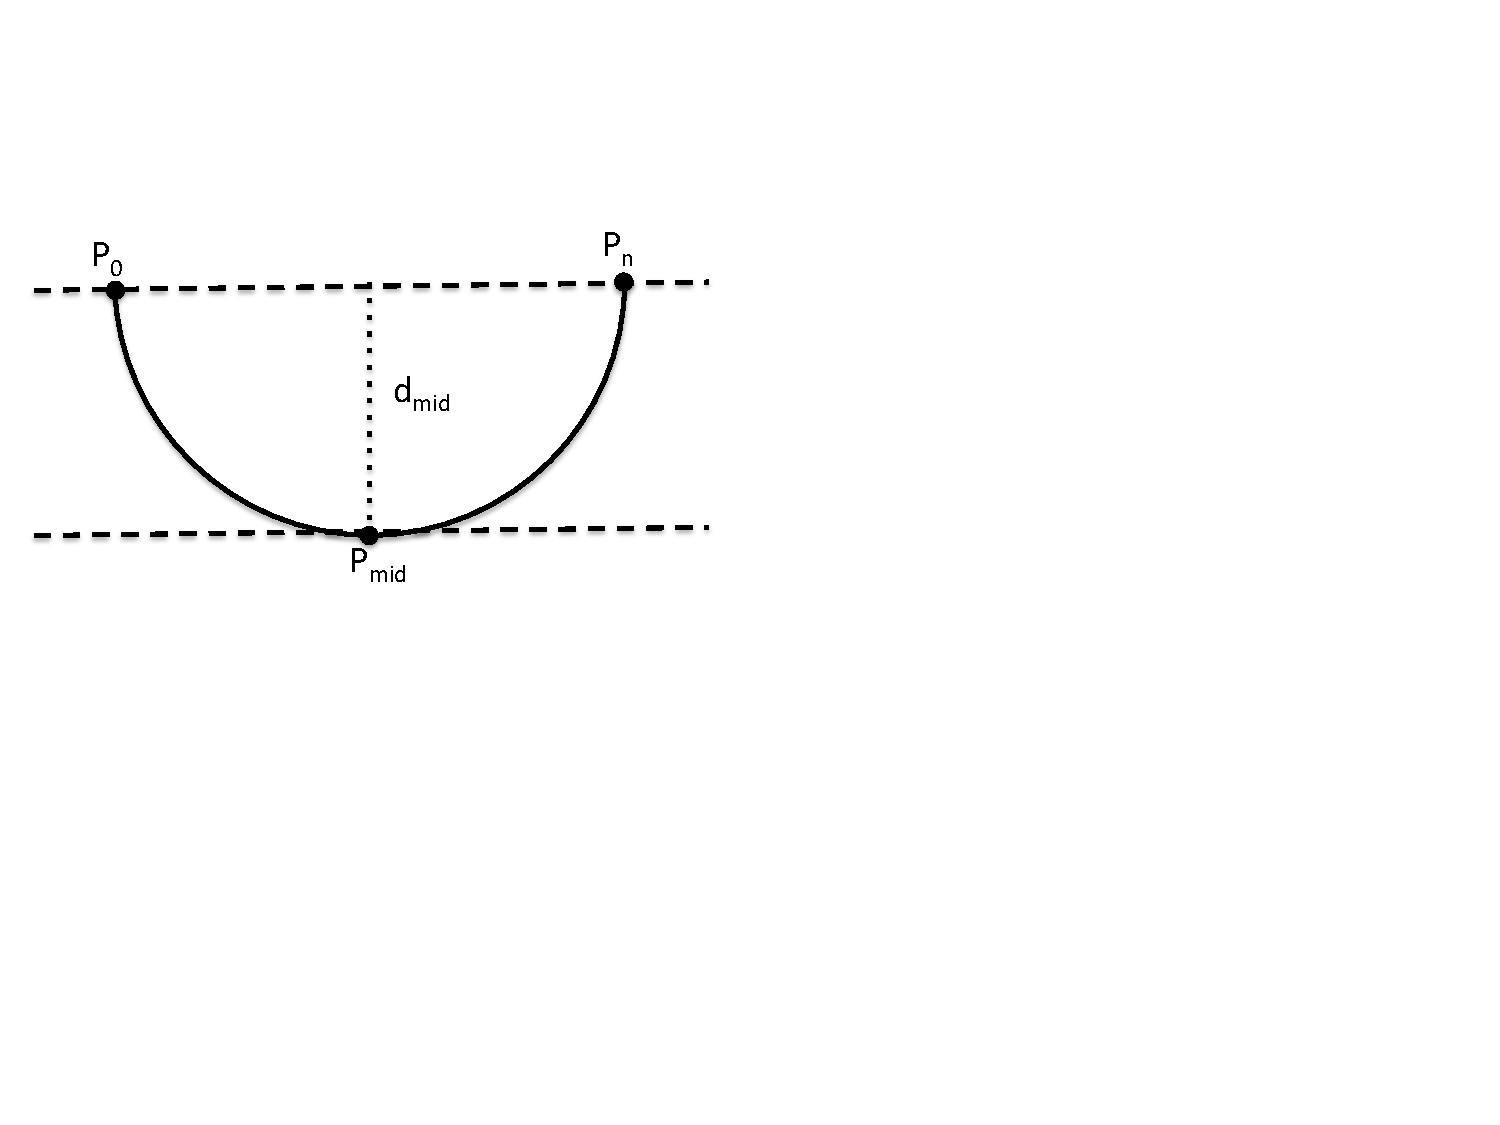
\includegraphics[width=\textwidth]{pics/circ1}   
    \caption{Circularity criterion in a perfect circle is: $|\overline{P_0P_n}|/d_{mid}=0.5$}
     \label{fig:circ1}
  \end{minipage}
  \hfill
  \begin{minipage}[b]{0.49\textwidth}
    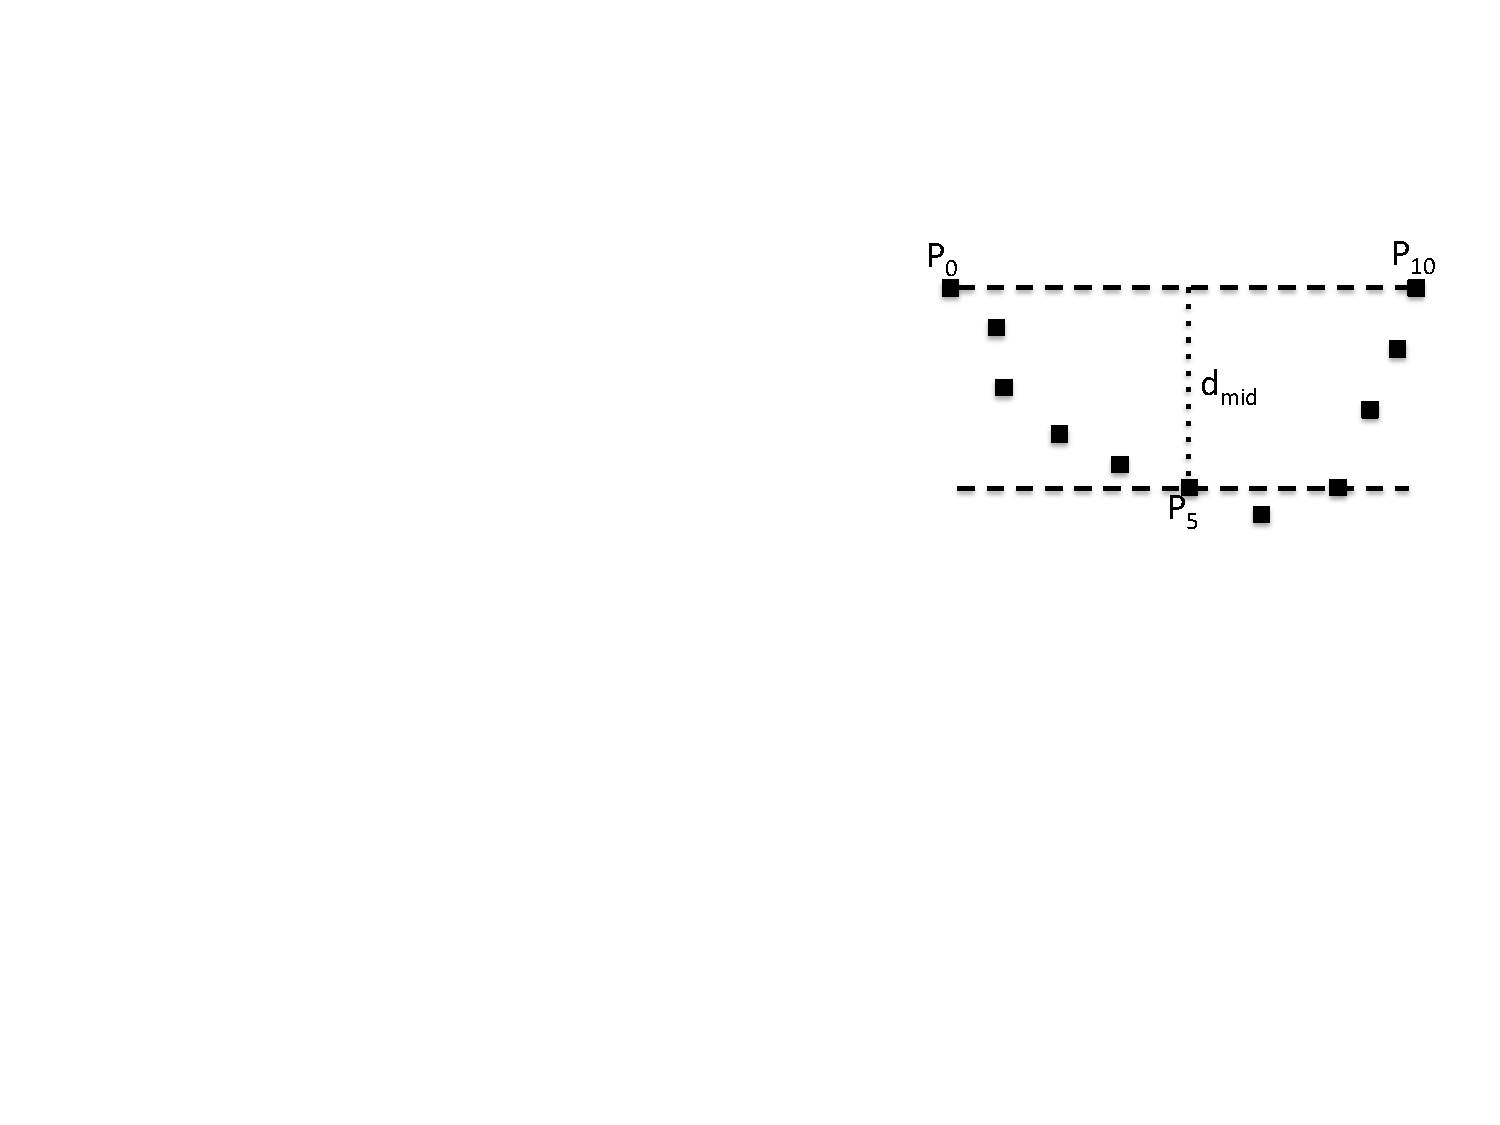
\includegraphics[width=\textwidth]{pics/circ2}    
    \caption{Circularity criterion in a this laser segment is: $|\overline{P_0P_{10}}|/d_{mid}=0.5$}
    \label{fig:circ2}
  \end{minipage}
\end{figure}

\item Inscribed Angle Variance (IAV): This feature is originally proposed by Xavier \cite{xavier2005fast}, in order to detect circles. For shapes that are not perfect circles but are similar to circles, IAV feature should be consistent. Laser segments from a leg usually resemble a circle, therefore we use IAV as one of the features for leg detection. As an example, inscribed angles on a circle is shown in Figure \ref{fig:iav}. As a geometric property of the circle, angles $\angle P_0P_1P_4$ and $\angle P_0P_2P_4$ are equal. IAV for a given set of points is the average of all inscribed angles: 
\[
IAV_S = \sum_{P = P_1}^{P_{n-1}} \dfrac{\angle P_0PP_n}{n}
\]
where $IAV_S=90^{\circ}$ for a perfect circle.

\begin{figure}[ht!]
\centering
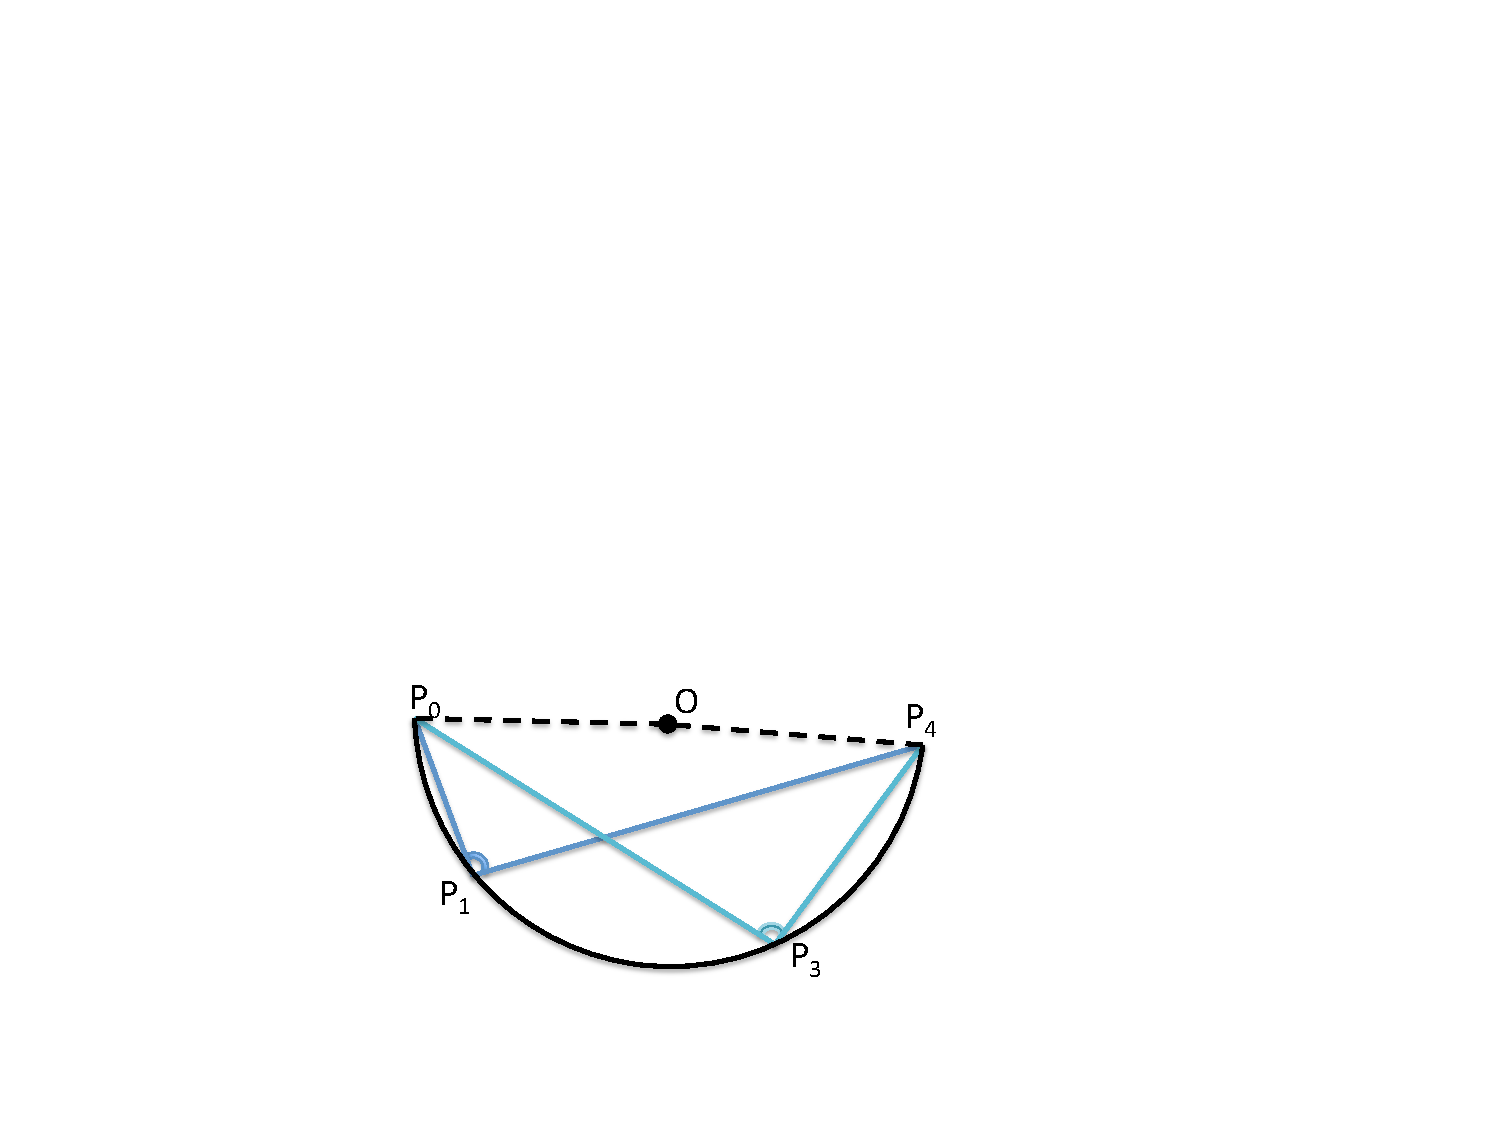
\includegraphics[width=0.4\textwidth]{pics/iav}
\caption{Inscribed angles of an arc are shown in the figure. Inscribed Angle Variance (IAV) is calculated by taking the average of all inscribed angles on a laser segment.}
\label{fig:iav}
\end{figure}

\end{enumerate}


For the training set, two people's legs were recorded with different clothing (shorts, baggy pants and trousers) to account for variance in the leg parameters. About $17\times 10^3$ Single Leg and $0.6\times 10^3$ person-wide blob patterns were manually labeled in the data. In addition, $120\times 10^3$ segments were labeled as 'other'. We first pre-computed the mean and standard deviation of these features, and then use these values for detection. We captured a set of laser scans data while the robot followed a person through an office environment. The following method used for this experiment will be discussed in detail in Section \ref{sec:following_basic_person_following}. The mean and standard deviations of geometric features for single leg, personwide blob, as well as other segments are given in Table \ref{table:leg_features}. 

\begin{table}
	\centering
  \begin{tabular}{lSSSSSS}    
    \toprule
    \multirow{2}{*}{Segment type} &
      \multicolumn{2}{c}{Width($m$)} &
      \multicolumn{2}{c}{Circularity} &
      \multicolumn{2}{c}{IAV($radians$)} \\
      & {$\mu$} & {$\sigma$} & {$\mu$} & {$\sigma$} & {$\mu$} & {$\sigma$} \\
      \midrule
    Single Leg & 0.13 & 0.03 & 0.25 & 0.15 & 2.23 & 0.4 \\
    Personwide blob & 0.33 & 0.07 & 0.14 & 0.09 & 2.61 & 0.16 \\
    Other & 0.22 & 0.12 & 0.1 & 0.11 & 2.71 & 0.38 \\
    \bottomrule
  \end{tabular}
      \caption{Table shows the mean and standard deviation of geometric leg features training set.}
    \label{table:leg_features}
\end{table}

For every segment $S_i$ in a test laser scan, we first extract the geometric features $f_1^i,f_2^i,f_3^i$. We then calculate the weighted Mahalanobis distance to the average leg parameters for the each leg pattern:
\begin{align}
\label{eq:mahalanobis}
D_{mah}^i=\sum_{j=1}^{n_{features}} w_j \frac{(f_j^i-\mu_j)^2}{\sigma_j^2}
\end{align}
where $w_j$ is the weight for each feature and $\mu_j$ and $\sigma_j$ are pulled from Table \ref{table:leg_features}. The resulting Mahalanobis distance $D_{mah}$ is then compared with a detection threshold. If $Dmah_{leg}^{i}< Threshold_{leg}$, the segment $S_i$ is considered a detection. $Threshold_{leg}$ defines how many standard deviations away from the average features are allowed. In our implementation, we empirically set the feature weights as:  $\textbf{W}_{leg} =(0.35, 0.26, 0.39)$, with the feature order given in Table \ref{table:leg_features}. For normal operation, we set  $Threshold_{leg}=1.5$, which accounts for about $\%95$ of the detections. If only one person is being tracked, we use a higher threshold. The reasoning behind this will be explained in Section \ref{sec:multimodal_person_state_estimation}.

\subsubsection{Associating Leg Segments}

After single leg patterns are detected, we attempt matching the leg segments by determining whether each leg pair are connected. The method described in this section applies to configurations where a RGB-D camera is pointing to the lower body of the human. For each leg segment pair, if both of them are within the FOV of the RGB-D sensor, we use our algorithm to determine whether there is a connectivity between two candidate leg segments. If connectivity is found, then the leg segments pair is qualified to be a leg segment pair representing a person. If this method is not applicable due to robot configuration, we use solely the distance between leg pairs for association. See Figure \ref{fig:leg_connectivity} as an example result. Figure \ref{fig:leg_connectivity_diagram} shows the flow chart of the association algorithm.

\begin{figure}[ht!]
\centering
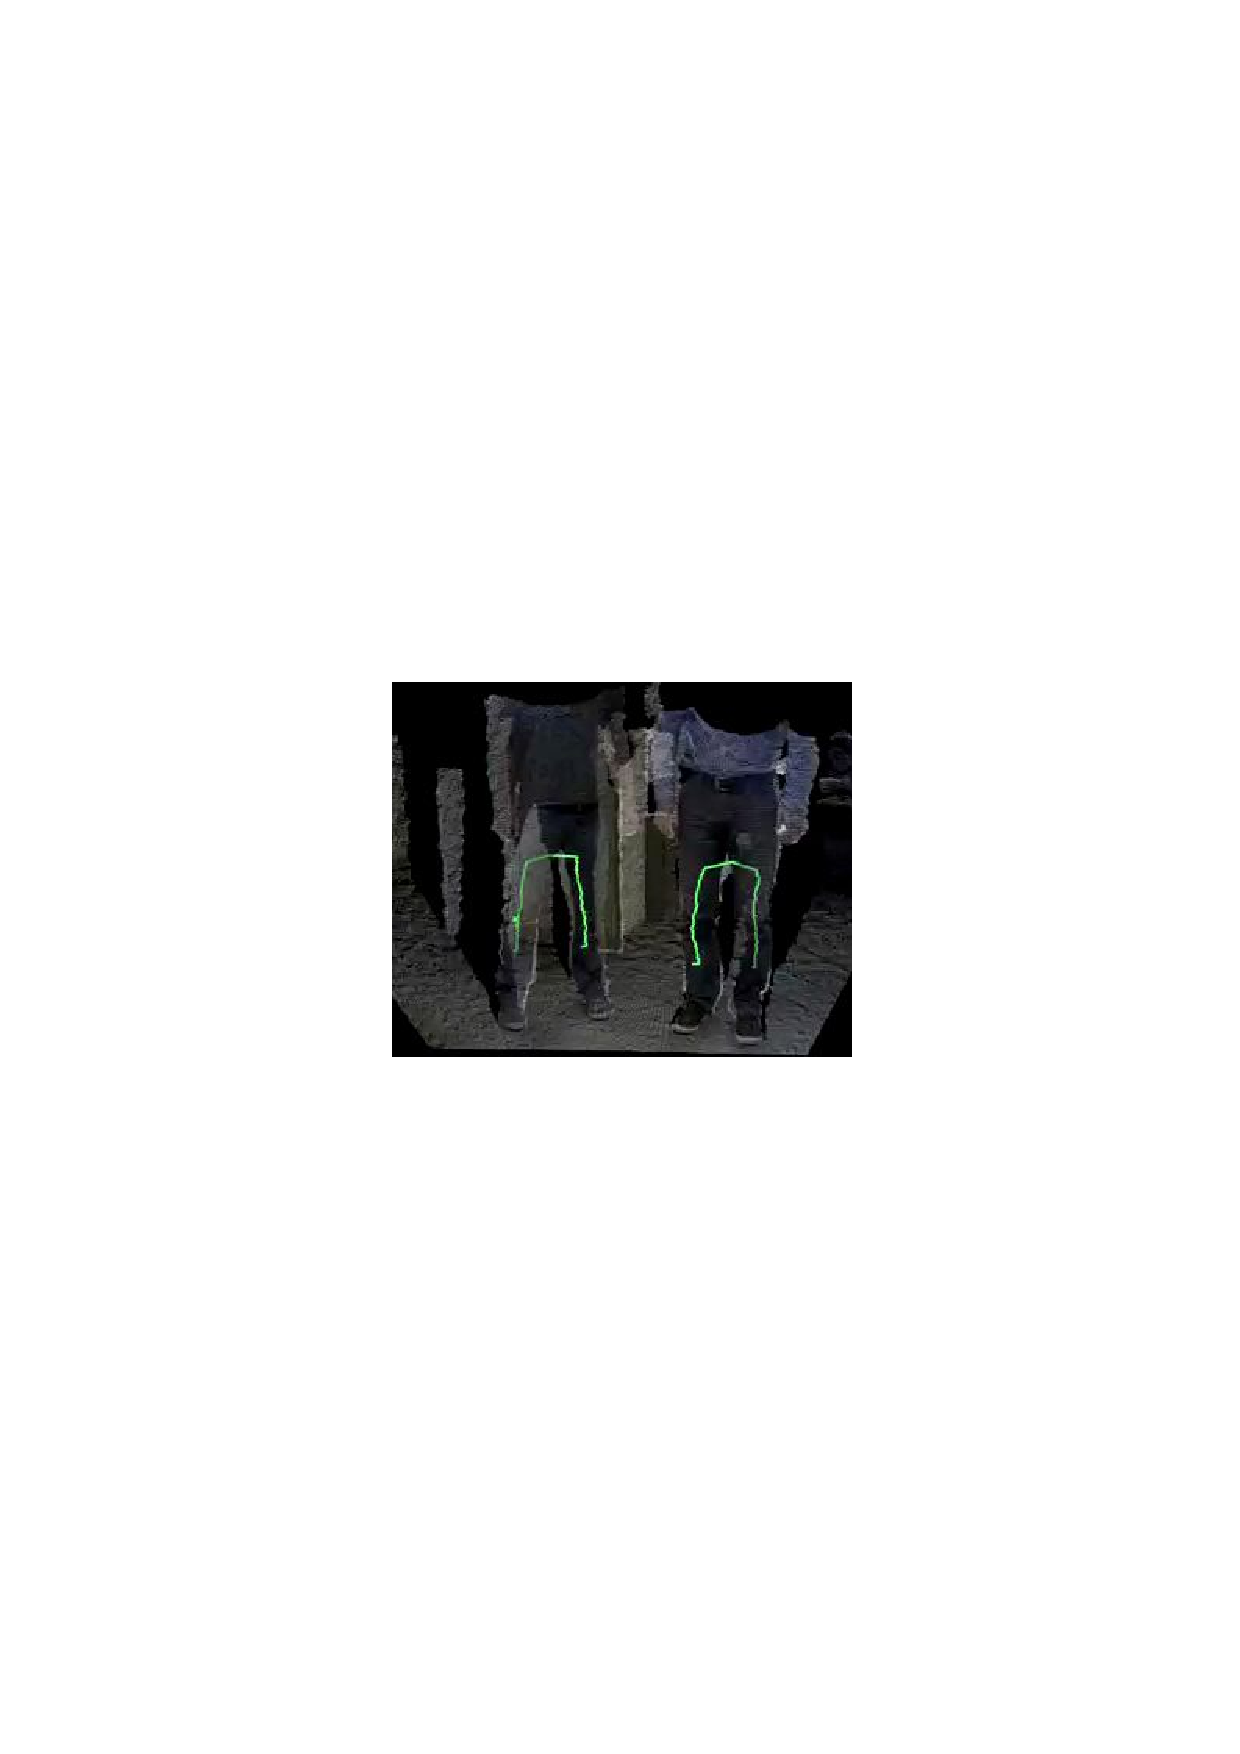
\includegraphics[width=0.6\textwidth]{pics/leg_connectivity}
\caption{Two person detections are seen in this figure. Our leg segment association algorithm propagates pixels vertically from candidate leg segments and connects leg pairs.}
\label{fig:leg_connectivity}
\end{figure}

\begin{figure}[ht!]
\centering
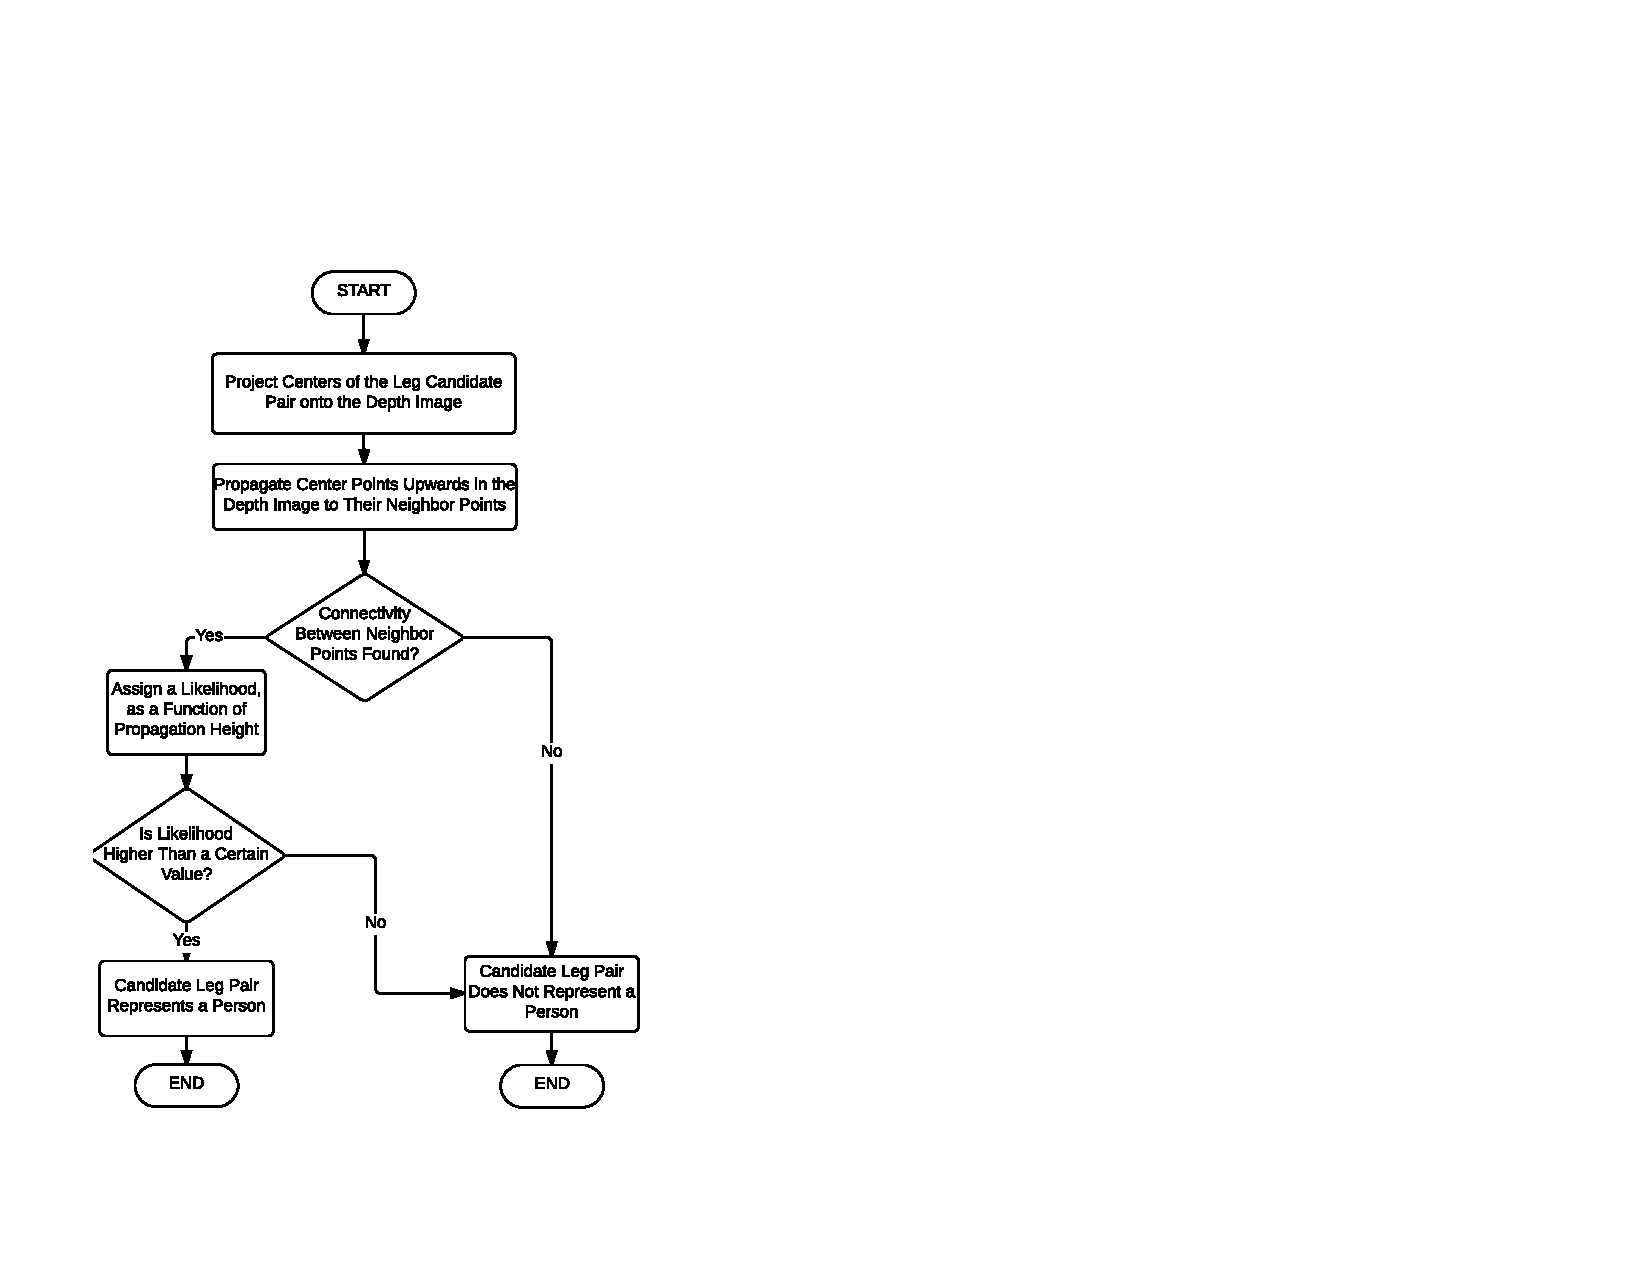
\includegraphics[width=0.5\textwidth]{pics/leg_connectivity_diagram}
\caption{Flow chart for determining if two leg segment candidates belong to a single person.}
\label{fig:leg_connectivity_diagram}
\end{figure}

First, the centroids each of the two candidate leg segments are found.  These points are projected onto the depth image acquired from the RGB-D camera. At each iteration for each leg segment, our algorithm first propagates horizontally to both directions in th e depth image to determine the center pixel, and it propagates 1 pixel vertically ($+z$ direction). If there are no connectivity after a number of iterations, then we conclude that the candidate leg pair does not represent a person. If there is a connectivity at some point, we then assign a likelihood score to the pair as a function of the vertical propagation height. If this score is higher than a threshold, then the algorithm concludes that the leg candidate segments represent a person. In our experience, we observed that the propagation scoring eliminates most of the false positives.

\subsection{Torso Detection}
\label{sec:multimodal_torso_detection}

For this detector, we used another Hokuyo UTM 30-LX laser scanner, placed at torso height ($1.27m$), aligned to the back of the robot. Our approach relies on fitting an ellipse to laser segments and interpreting the axis lengths. By using the shape of the ellipse, it is estimate to infer the orientation of the person. (Figure \ref{fig:ellipse}).

\begin{figure}[ht!]
\centering
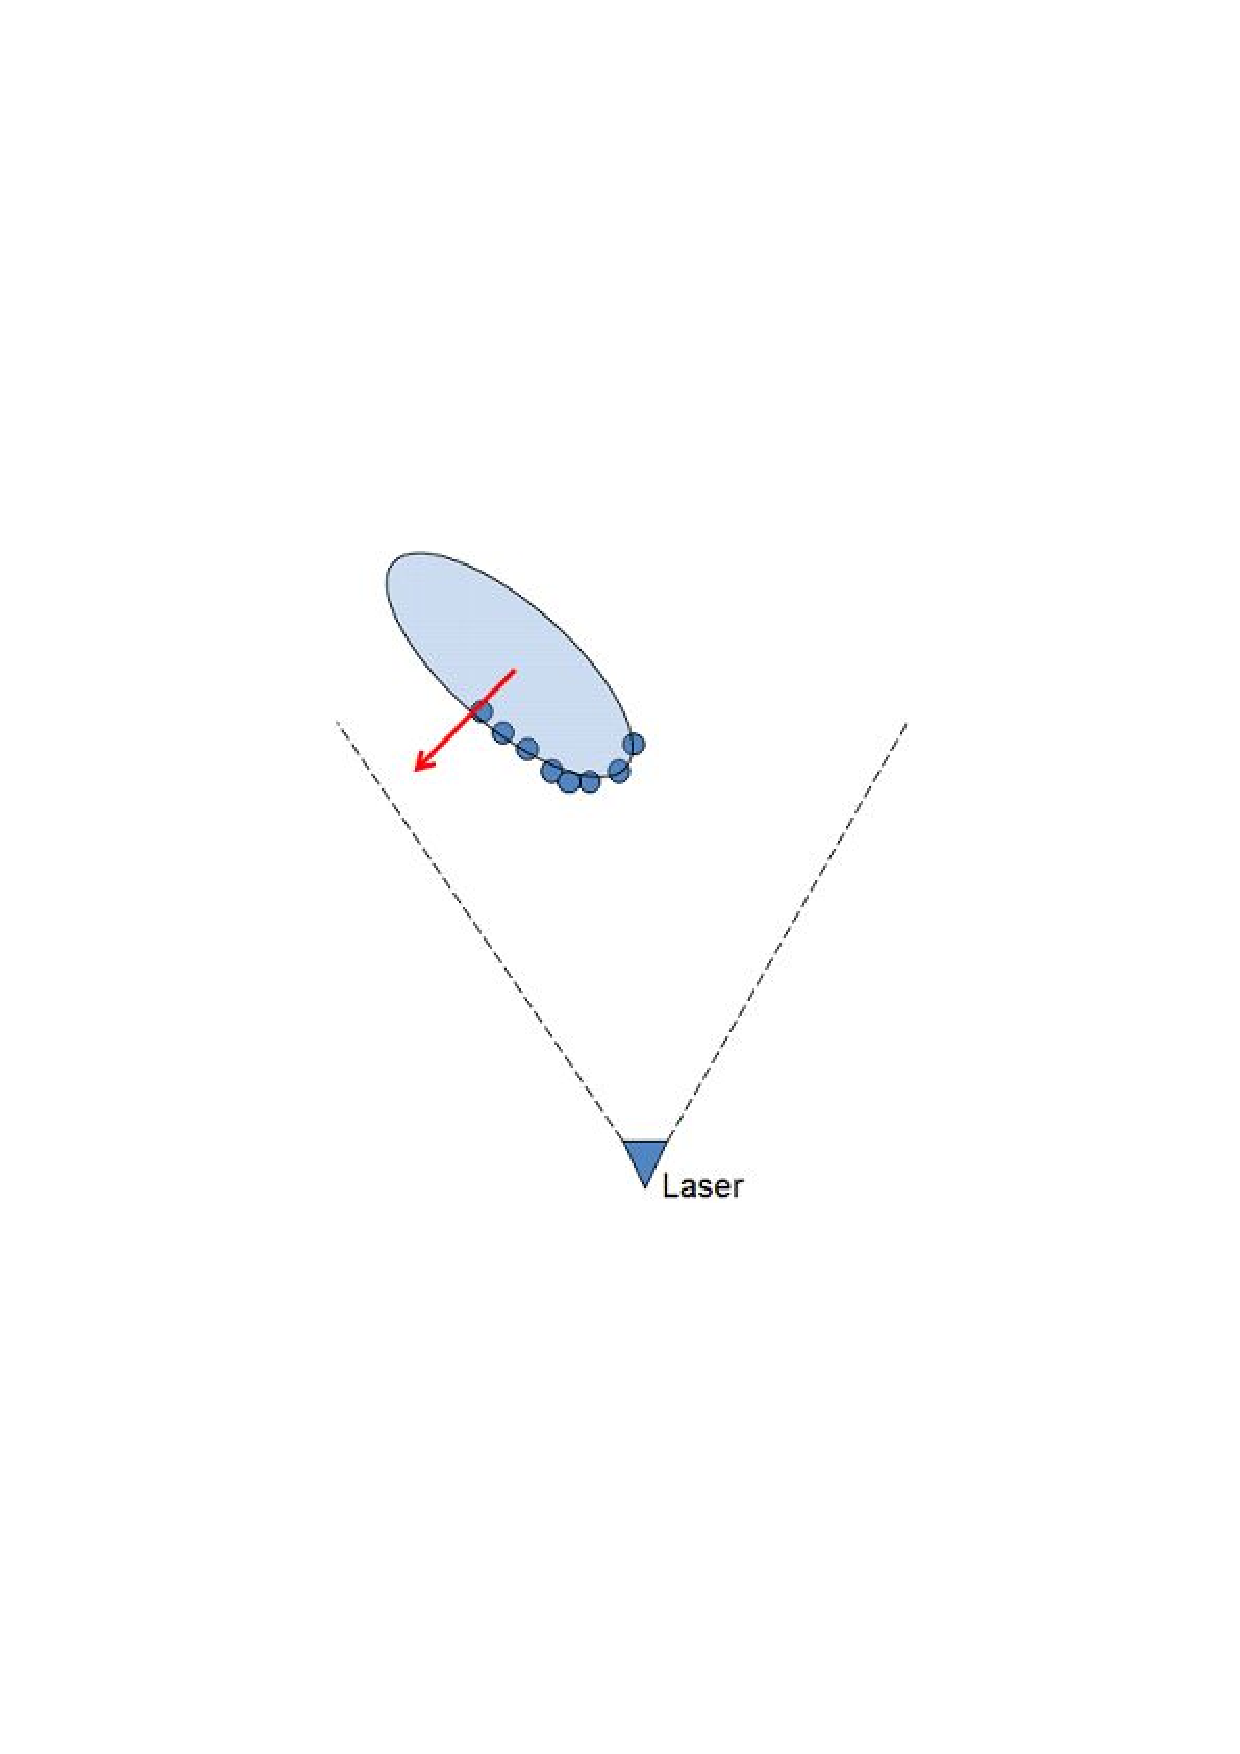
\includegraphics[width=0.35\textwidth]{pics/ellipse}
\caption{Our torso detector fits an ellipse to the human torso and estimate its position and orientation using the ellipse centroid and axis lengths.}
\label{fig:ellipse}
\end{figure}

The first step to detect torsos in a laser scan is to segment the laser scan into clusters. We use the same segmentation technique used for leg detection, as explained in Section \ref{sec:multimodal_leg_detection}. We then fit an ellipse to each laser segment. We use a numerical ellipse fitting method that solves the problem with a generalized eigensystem, introduced by Fitzgibbon \cite{fitzgibbon1999direct}. This fitting method is robust, efficient and ellipse-specific, so that even very noisy sensor data will always return an ellipse. Compared to iterative methods, it is computationally more efficient.

To detect a torso in a laser segment, we use the minor and major axis lengths, in addition to the three geometric features introduced in Section \ref{sec:multimodal_leg_detection} for detection of legs. We collected 450 laser scans while a person stood $2m$ away from the sensor and made a one full turn around. We calculated the mean and standard deviation of the all five features, which is given in Table \ref{table:torso_tracking_results}. For a given laser segment, we find the weighted Mahalanobis distance in Equation \ref{eq:mahalanobis} to the averaged parameters. If $Dmah_{torso}^{i}< Threshold_{torso}$, the segment is considered a detection. The feature weight constants we used was $\textbf{W}_{torso} =(0.19, 0.09, 0.35, 0.24, 0.13)$, in respective order given in Table \ref{table:torso_feature_averages}. These values were empirically determined, although it is possible that optimizing the feature weights would yield better results.

\begin{table}
	\centering
  \begin{tabular}{lSSSSSS}    
    \toprule
    {Torso Features}
      & {$\mu$} & {$\sigma$} \\
      \midrule
    Width($m$) & 0.44 & 0.12 \\
    Circularity & 0.32 & 0.18 \\
    IAV($radians$) & 2.57 & 0.38\\
    Major axis length($m$) & 0.39 & 0.08\\
    Minor axis length($m$) & 0.17 & 0.06\\
    \bottomrule
  \end{tabular}
      \caption{Table shows average and standard deviations of geometric features for a human torso in laser scans.}
    \label{table:torso_feature_averages}
\end{table}

Figure \ref{fig:torso_detection_rate} shows how the torso detection success rate vs Mahalanobis Distance Threshold in our dataset. What is not displayed in the plot is that a higher detection threshold leads to more false positive rates. For normal operation, we set $Threshold_{torso}=1.25$, which accounts for about $\%90$ detection rate. If the tracker is dedicated to track only a single person, then we use a higher threshold, $Threshold_{torso}=2$, to account for about $\%99$ of the detections. The reason for a higher threshold is that false positives would be dismissed anyway if only a single person is tracked.

\begin{figure}[ht!]
\centering
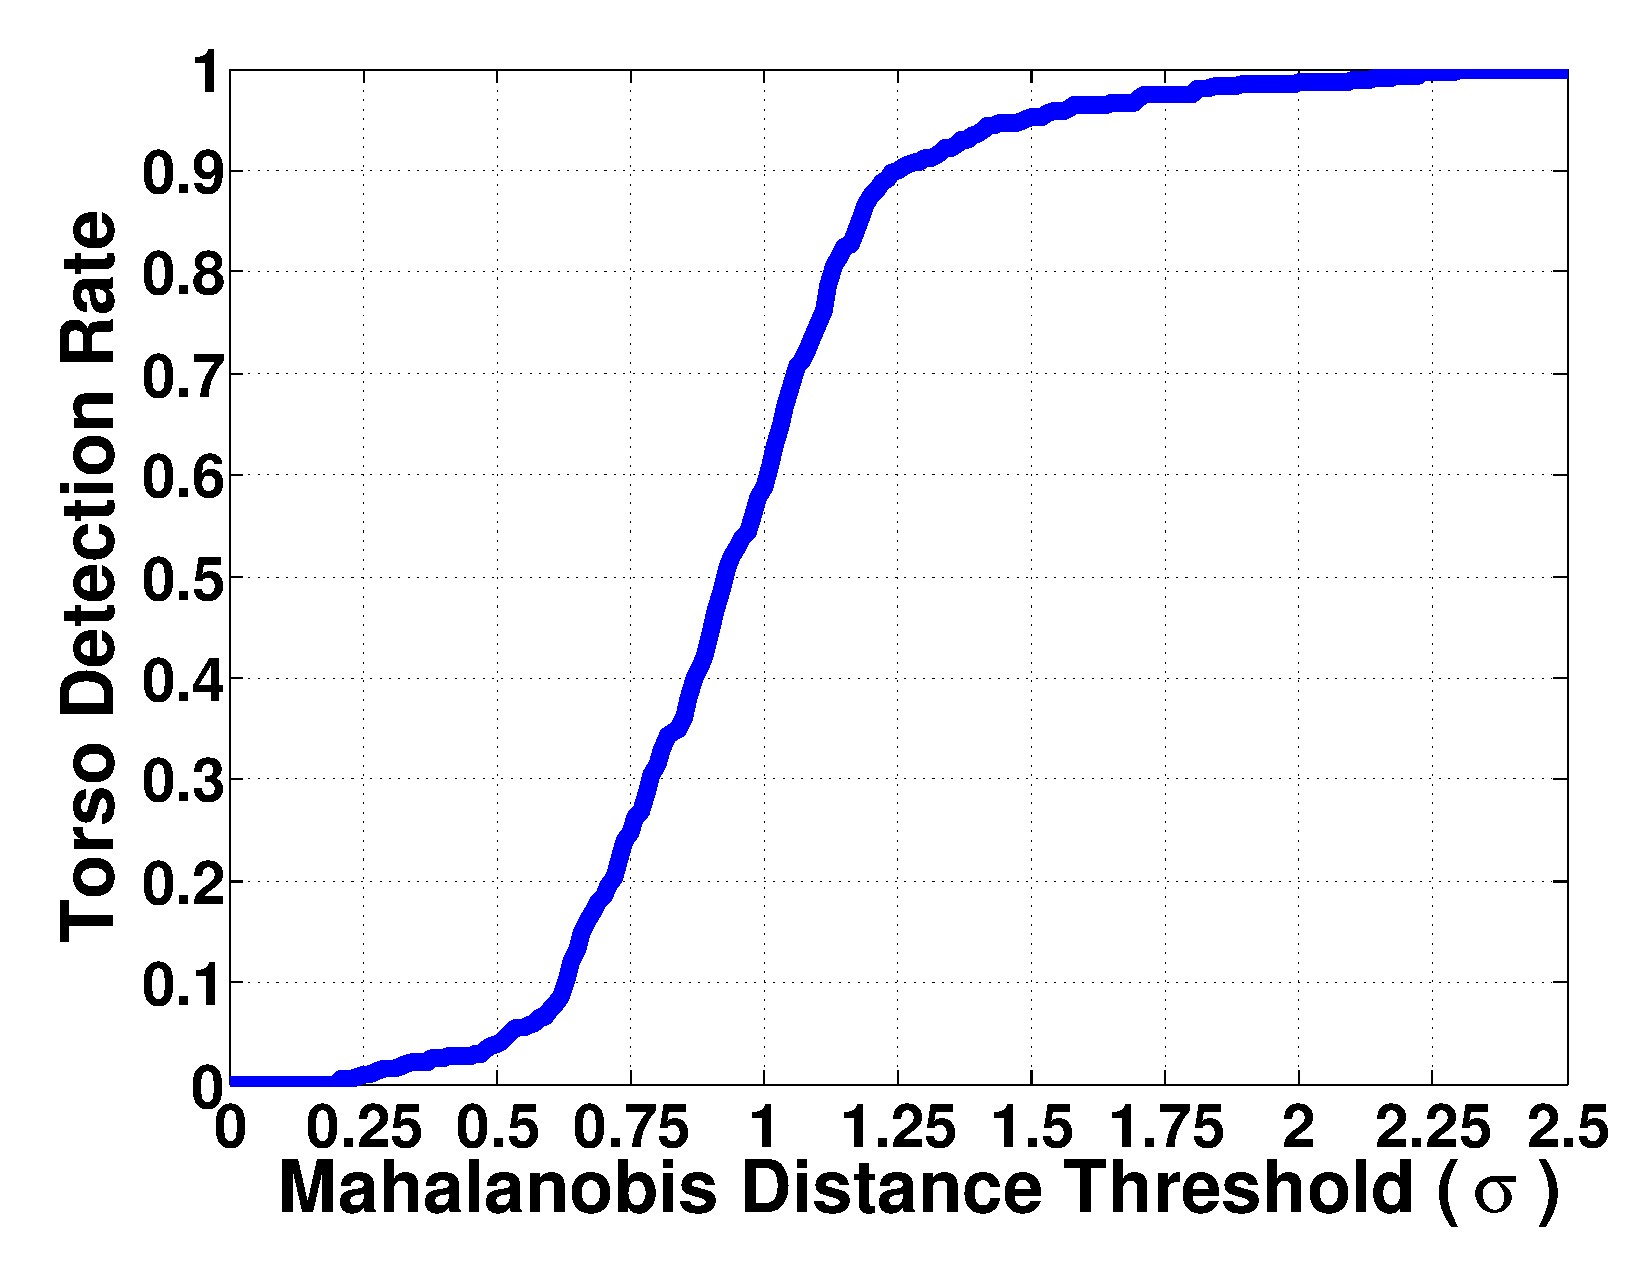
\includegraphics[width=0.6\textwidth]{pics/torso_detection_rate}
\caption{Torso detection rate vs the detection threshold}
\label{fig:torso_detection_rate}
\end{figure}

\subsubsection{Evaluation of Torso Detection}

The ellipse fitting algorithm output is the centroid of the ellipse, and the minor and major axes. We assume the orientation of detected humans is aligned with the minor axis. This provides two solutions: either the front or the back of the person is visible to the sensor. While this is a significant limitation our current system, one can potentially utilize face detection as will be described in Section \ref{sec:multimodal_face_recognition} to estimate if the person is facing the front of the robot or not.

In order to evaluate the accuracy of the position and orientation estimations of our torso detection method, we collected torso data from 23 people. Subjects were instructed to stand on 4 targets at different distances with 8 different orientations on each target. Experimental setup from the sensor's point of view is shown in Figure~\ref{fig:torso_tracking_exp_setup}. For each pose at every target, we logged the position and orientation estimation of the torso detector and compared it with ground truth, which is defined by the markings on the floor.

\begin{figure}[h]
\centering
        \subfigure{%
            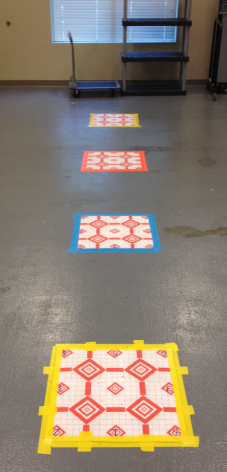
\includegraphics[width=0.2\textwidth]{pics/exp0}
        }%
        \subfigure{%
            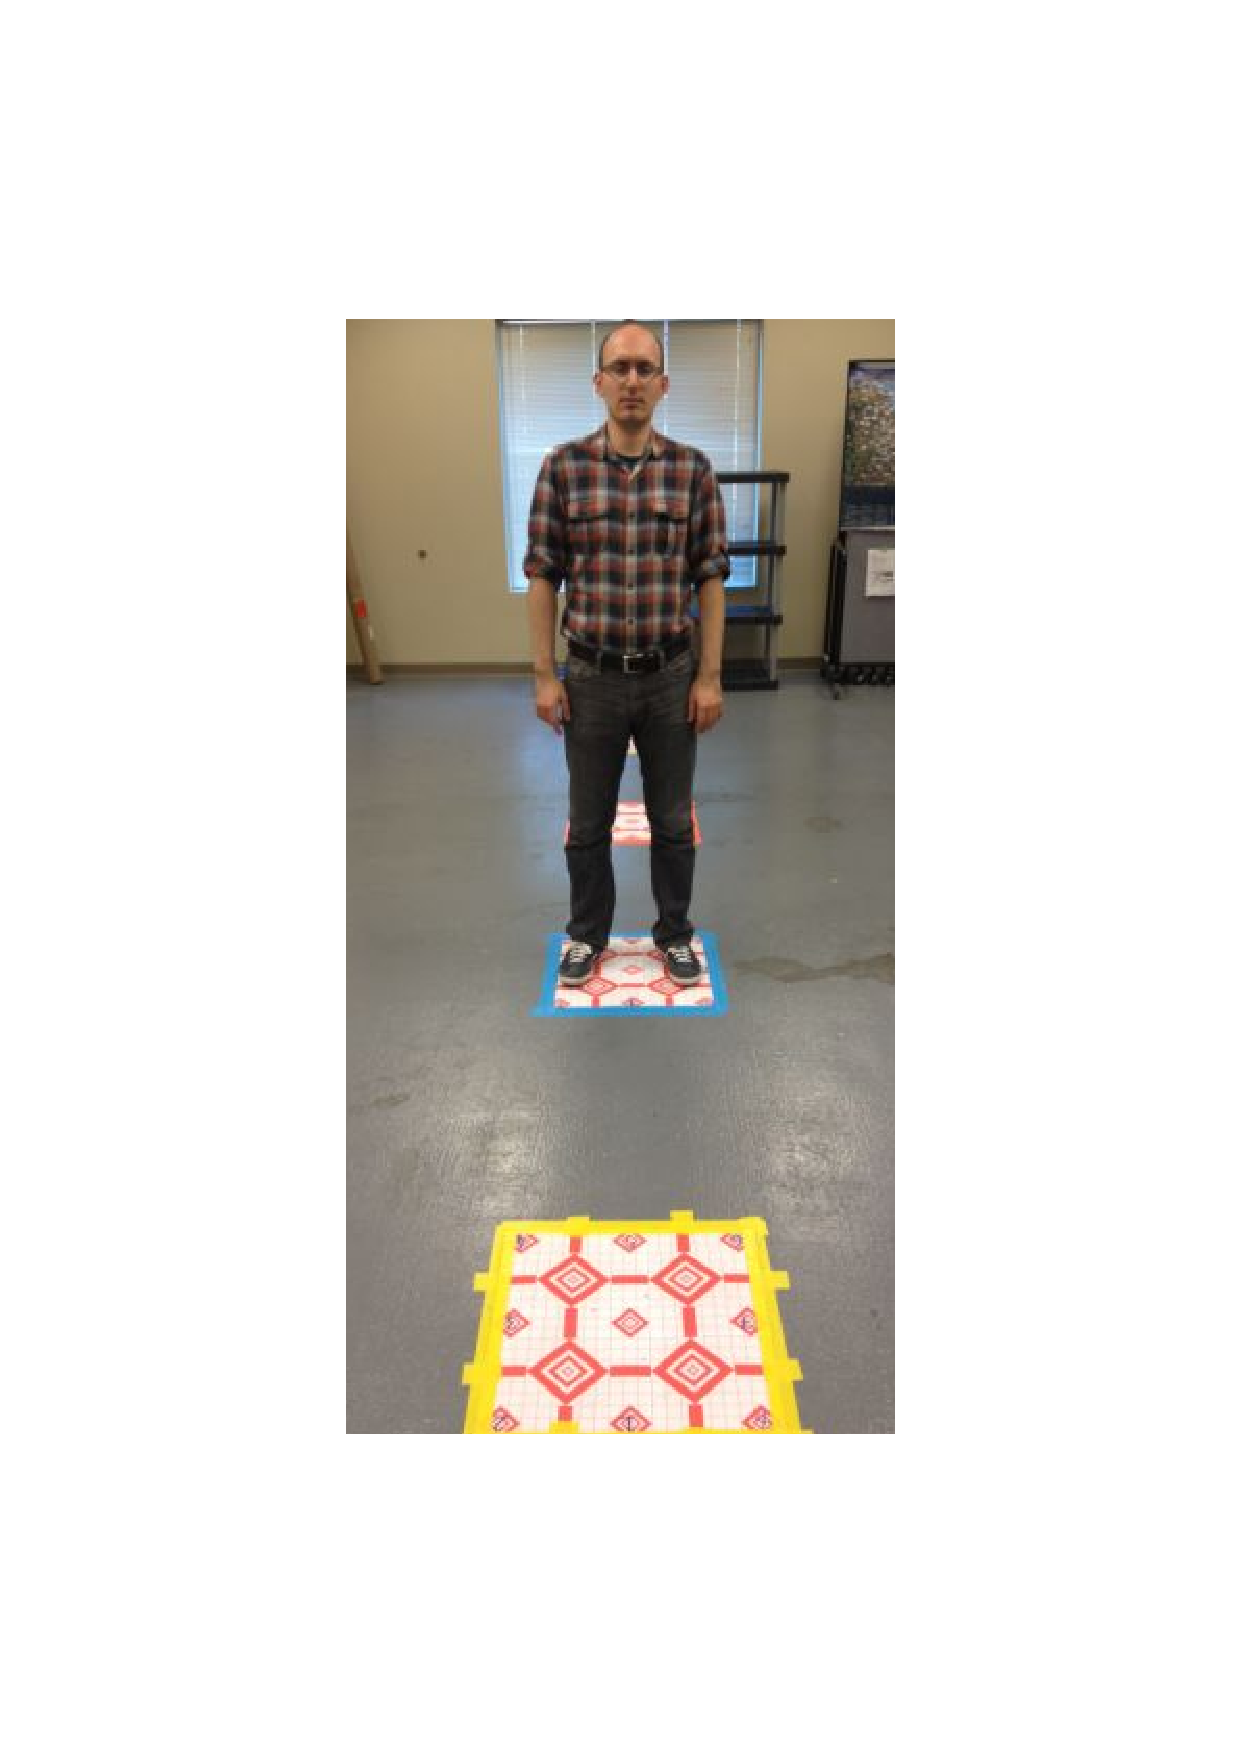
\includegraphics[width=0.211\textwidth]{pics/exp1}
        }%
        \subfigure{%
           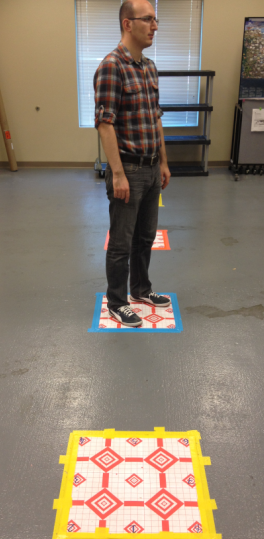
\includegraphics[width=0.205\textwidth]{pics/exp2}
        } %  ------- End of the first row ----------------------%
        \subfigure{%
           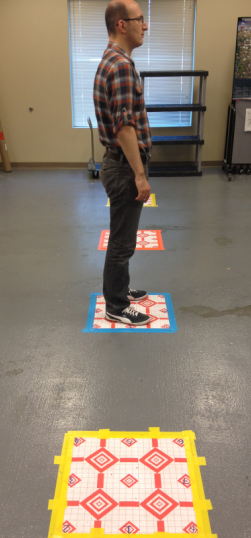
\includegraphics[width=0.197\textwidth]{pics/exp3}
        }\\ %  ------- End of the first row ----------------------%
    \caption{%
	Experimental setup for measuring the position and orientation estimation errors of torso detection. The pictures are taken from the laser scanner's point of view.
     }%
   \label{fig:torso_tracking_exp_setup}
\end{figure}


Table~\ref{table:torso_tracking_results} shows the angular error at every target distance and human orientation with respect to the laser scanner. 

\begin{table}[ht!]
\centering
\begin{tabular}{cSSSSSSSSS}    
 \toprule 
Distance To Laser & {N} & {NE} & {E} & {SE} & {S} & {SW} & {W} & {NW} & {ALL}\\
\midrule
{$1.0m$} & {$4^{\circ}$} & {$12^{\circ}$} & {$22^{\circ}$} & {$13^{\circ}$} & {$5^{\circ}$} & {$7^{\circ}$} & {$26^{\circ}$} & {$17^{\circ}$} & {$13^{\circ}$} \\
{$2.5m$} & {$5^{\circ}$} & {$16^{\circ}$} & {$19^{\circ}$} & {$10^{\circ}$} & {$3^{\circ}$} & {$6^{\circ}$} & {$14^{\circ}$} & {$17^{\circ}$} & {$11^{\circ}$} \\ 

{$4.0m$} & {$4^{\circ}$} & {$10^{\circ}$} & {$30^{\circ}$} & {$16^{\circ}$} & {$7^{\circ}$} & {$11^{\circ}$} & {$21^{\circ}$} & {$17^{\circ}$} & {$15^{\circ}$} \\ 
{$5.5m$} & {$5^{\circ}$} & {$11^{\circ}$} & {$41^{\circ}$} & {$18^{\circ}$} & {$10^{\circ}$} & {$6^{\circ}$} & {$38^{\circ}$} & {$23^{\circ}$} & {$19^{\circ}$} \\ 

{ALL} & {$4^{\circ}$} & {$12^{\circ}$} & {$27^{\circ}$} & {$14^{\circ}$} & {$6^{\circ}$} & {$7^{\circ}$} & {$24^{\circ}$} & {$18^{\circ}$} & {$14.5^{\circ}$} \\
\bottomrule
\end{tabular}
\caption{Mean orientation error of the torso detector with respect to distance from sensor and body pose is shown. Data from 23 individuals are used.}
\label{table:torso_tracking_results}
\end{table}

The average position error was about $5cm$ regardless of the distance and the orientation of the human. The average orientation error throughout all the experiments was $14.5^{\circ}$. Error in orientation, however, varied greatly by the pose of the person with respect to the laser scanner. Average error in orientation differed slightly with respect to the distance from the sensor and was the least with $11^{\circ}$ when the humans were $2.5m$ away from the sensor. We attribute to the fact that when humans closer than $2.5m$ to the laser scanner, it captures more of the arms, which makes the fitted ellipse slightly worse. The orientation of the human with respect to the sensor had a significant effect on orientation error. Least error was achieved when people faced the sensor  ($4^{\circ}$) or the opposite way ($6^{\circ}$). On the other hand, average orientation error was $24^{\circ}-27^{\circ}$ when humans are perpendicular to the sensor, because a large portion of the torso is not visible to the laser scanner in that configuration.

\section{Person State Estimation}
\label{sec:multimodal_person_state_estimation}

The position and velocity of the person can not be determined by direct observation due to measurement noise and false detections. Therefore there is a need for a filtering algorithm in order to estimate the state of a person. Using a state predictor for human movement has two advantages. First, the predicted trajectories are smoother than raw detections. Smooth tracking helps the robot maintain consistent trajectories for high-level applications such as Person Following (Section \ref{chapter:person_following}). Second, it provides a posterior estimation that can be used for data association when there is a lack of matching detections. This allows the tracker to handle temporary occlusions. We use a discrete Kalman Filter \cite{kalman1960new} to predict the position and velocity of a person. There are other types of filtering techniques available in the literature, such as Particle Filters \cite{khan2004mcmc}. Since the results of the person state estimator is used by time-critical higher level applications, the tracker should come up with an estimate in real time. Therefore the choice of using Kalman Filters was motivated by its computational efficiency. Efficient person state estimation also increases the safety of the robot, as the robot can react faster if there are people in close proximity.

Accoding to Hicheur \cite{hicheur2005velocity}, humans tend to maintain a constant speed when they are walking straight and reduce speed while turning. Using this observation, we used constant velocity model which assumes people will maintain their speed. Even though this assumption is not always true, it provides a simple model without sacrificing too much from tracking performance.

The Kalman filter estimates a process as a predictor-corrector cycle using feedback control. The process has two cycling states: time update and measurement update. Time update projects the state forward by using the current state and error covariance. Measurement update is responsible for the feedback and corrects the previous estimate.

The Kalman Filter is governed by two linear stochastic difference equations:
\begin{align}
s_k&=As_{k-1}+Bu_{k-1}+w \\
z_k&=Hs_k+v
\end{align}

Where $s_k$ represents the process state at time step $k$, $A$ is the state propagation matrix, $B$ relates the optional control input $u$, $z_k$ is a measurement, $H$ is the measurement observation matrix. $w$ and $v$ represent the process and measurement noises, respectively, drawn from normal probability distributions with zero mean $N(0,Q)$ and $N(0,R)$.

We define the state of a person $s_k$ at time step $k$ as:
\begin{align}
s_k & =
\begin{bmatrix} 
 x_k \\ 
 y_k\\
 \dot{x}_{k} \\
 \dot{y}_{k}
\end{bmatrix}
\end{align}

where $(x_k,y_k)$ is the position and $(\dot{x}_{k}, \dot{y}_{k})$ is the velocity of the person in Cartesian Coordinates. With the constant velocity model, the time update equations are:
\begin{align}
x_k&=x_{k-1}+\dot{x}_{k-1} \Delta t_k\\
y_k&=y_{k-1}+\dot{y}_{k-1} \Delta t_k\\
\dot{x}_{k}&=\dot{x}_{k-1} \\
\dot{y}_{k}&=\dot{y}_{k-1}
\end{align}
where $\Delta t_k$ is the time difference from the previous detection. This results in the following Kalman Filter matrices:
\begin{align}
A =
\begin{bmatrix} 
 1 & 0 &\Delta t_k & 0\\
 0 & 1 & 0 & \Delta t_k\\
 0 & 0 & 1 & 0\\
 0 & 0 & 0 & 1
\end{bmatrix} &&
B =
\begin{bmatrix} 
 0 \\
 0 \\
 0 \\
 0
\end{bmatrix} &&
H =
\begin{bmatrix} 
1 & 0 & 0 & 0 \\
 0 & 1 & 0 & 0
\end{bmatrix} 
\end{align}
A track is lost if there are no detections for a fixed amount of time. At every time update of a filter, if $\Delta t_k$ is larger than a fixed threshold, the track is killed.

The reason $B$ vector is zero is that we track people in the world frame and robot motion is already accounted for with robot localization. For this reason, we assume there are no control inputs to our system. The noise matrices we used are:
\begin{align}
Q=qI_4
&&
R=rI_2
\end{align}

where we used $q=0.02$ and $r=1.0$ in practice.

Our approach is multimodal in the sense that asynchronous measurements are accepted from different sources as long as they provide a position estimate in the respective sensor frames. Using the latest localization information, this position is converted to the world frame. Before the measurement is accepted as valid, we execute one more check. We check if a new detection is in collision with the static map, and if it is in collision, we reject that detection. The check against the static map is fast and helps reduce false positives in practice. We use Nearest Neighbor (NN) data association \cite{bar1995multitarget}, which is a reasonable compromise between performance and computational cost. 

Depending on the task, a single person or multiple people must be tracked. For example, for following a person or guiding a person, tracking a specific user is sufficient. However, for point-to-point navigation or when searching a specific person, the robot should track multiple people. We examine each case below:

\begin{itemize}
\item \textbf{Single target tracking:} For some tasks, such as person following, dedicated tracking of a single specific user is required and tracking bystanders is optional. In this case, our goal is to keep tracking the specific user, so we significantly relax the detection thresholds of the detectors. Even though doing so results in more spurious detections, we do not start more than a single track. This approach improves the tracking performance of a single person.
\item \textbf{Multi-target tracking:} When the robot is navigating from a point to another among people, the robot should keep track of bystanders and respect their personal spaces. In multi-target case, we keep a separate Kalman filter for each tracked person. If a detection is matched to multiple tracks, only the closest track is associated with the detection and the other filters are considered to have no detections for that time step.
\end{itemize}

\section{Face Recognition}
\label{sec:multimodal_face_recognition}

For certain interactive navigation tasks such as finding a specific person, a robot needs to have person recognition capability. Our person recognition approach uses face recognition and optionally shirt color features. We detect faces in RGB images using the popular face detector by Viola and Jones \cite{viola2004robust}, and use the Eigenface method by Turk and Penland \cite{turk1991face}.

With the $Eigenface$ approach, face are represented in a lower-dimensional space. Sirovich and Kirby \cite{sirovich1987low} showed that dimension reduction method Principal Component Analysis (PCA) can be used on face images to form a set of basis features. The main idea of PCA for faces is to find vectors that best account for variation of face images in all training images. These vectors are called $eigenvectors$. Then a face space is constructed called $eigenfaces$ and the images are projected onto this space. Our approach of face recognition has the following steps:

\begin{figure}[ht!]
\centering
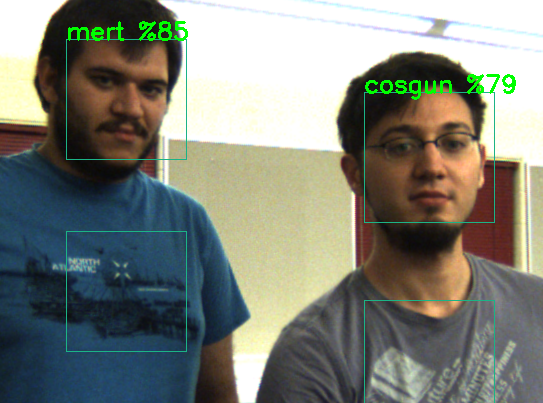
\includegraphics[width=0.6\textwidth]{pics/person_recognition}
\caption{Example results of our person recognition method is shown in the image. We use $Eigenfaces$ face recognition method and optionally shirt color recognition.}
\label{fig:person_recognition}
\end{figure}

\begin{enumerate}
\item A person previously unknown to the robot initiates training.
\item Robot asks the person to turn his face one side to another, and takes $M$ number of face and shirt pictures
\item Eigenfaces from the entire training set is calculated, and every known face is projected to the corresponding $M$-dimensional weight $facespace$.
\item After training is completed, face recognition is reactivated.
\item When face recognition is active, a distance value from face recognition and optionally from shirt color matching is received and it is thresholded for a decision.
\end{enumerate}

An example recognition result is shown in Figure \ref{fig:person_recognition}. Our approach allows new faces to be trained on-the-fly. Using the GUI of the robot, a user can start training and adjust the information in the person database. The person data is managed by a SQLite database hosted locally on the robot.

Shirt color matching can be used when there is not much time between the training and recognition. Activating the shirt color matching should improve recognition and reduce false positive detections. We take a rectangular region below the face as the shirt area ($1.5$ times below the the face rectangle size). A histogram with a number of bins is generated for each shirt pattern. Each pixel is pushed into bins according to their normalized RGB value. We calculate a distance value between two histograms using the Earth Mover Distance \cite{rubner1998metric}. In addition, the trained histogram can adaptively be updated at every high confidence detection in order to account for illumination changes. The overall person score is calculated by a weighted average of face and shirt distance.

%A possible use of person recognition in interactive navigation is to drive up to a specific person. Another possible use case for our work is to re-initialize person following if the user is lost. We have used face recognition in some of our applications, however it requires the face of the person to be visible. Vision community works on datasets that are selected nicely as pictures taken by humans are likely to have more faces in it. On the other hand, most frames the robot acquires won't have any faces in it. Development of person recognition approaches that are suited for on-board sensing on mobile systems is an open research area.
